\chapter{Poroelastic natural coatings}

\section{Biomimetics of poroelastic coatings}

Usually when someone is asked to imagine some "rapid" object as an airplane, a boat or a car, the common sense lead us to think about it as the smoothest as possible and most of the time shiny.
But if we look around us the nature seems not to agree with the previous statement.
In fact most of the surfaces in nature are not smooth at all, they present almost always some kind more or less regular arrangement of discontinuities at various length scales.
Since Nature have had a very large time-span to optimize this kind of surfaces we can be very certain that they are the best possible option.
One should pinpoint that the non smoothness of these surfaces can be connected to some other biological functions rather than pure fluid dynamic performance, and of course it can be the case.


With that in mind we want to show to the reader some of the most notably examples of "natural" aerodynamically surfaces.

Probably the most notable example is the shark skin, in figure \ref{fig:shark} a segment of the skin is depicted as if appears to be under the microscope.

\begin{figure}[h]
	\centering
	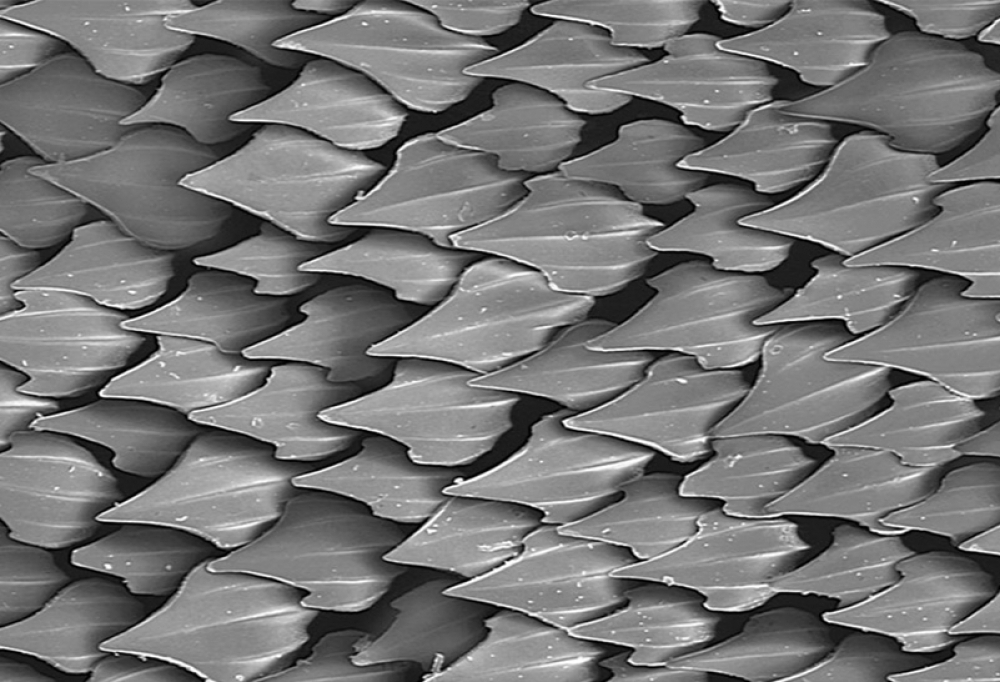
\includegraphics[width=0.5\linewidth]{chapter_1/shark}
	\caption{Microscope enlarged picture of the shark skin.}
	\label{fig:shark}
\end{figure}

The enlargement show that the surface is made up by a series of overlapped denticles, and experiment shows that they can move and interact with the flow.

The shark technology has somehow been applied by Speedo$^{\circledR}$ in their famous swimming suits, that had break multiples world records.
But it seems that this controversial swimmers performance came more on the compressed and streamlined body shape than from the surface texture itself.
In fact during the years this texture material has been publicized to be like synthetic shark skin but \cite{Oeffner785} has shown that the texture is somehow different from the shark dermal structure.
They have also performed some swimming experiment with a flat plate with different surfaces and they have found no significant speed enhancement with the swimsuit surfaces; but the measurements with the shark skin on the contrary give an appreciable improvement in the performance.


Poroelastic surfaces find also applications in aeroacoustics, in fact the owl is well known for its particularly silent flight, in the high frequency spectrum.
This characteristic is crucial for the owl in order to be able to capture his preys.
Obviously it has inspired the scientific community to study the feathers configuration and their shape.

\begin{figure}[h]
	\centering
	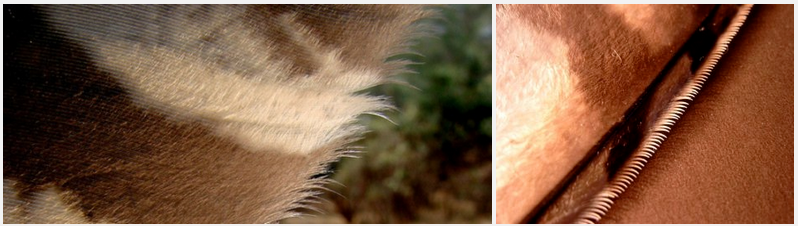
\includegraphics[width=0.7\linewidth]{chapter_1/howl}
	\caption{Feathers in owl's wing: trailing edge (left), leading edge (right). The difference in shape, and mechanical properties as rigidity, between the leading and trailing edge is a consequence of the different flow regimes in the wing.}
	\label{fig:owl}
\end{figure}
 
Multiple authors show promising result in characterizing the acoustic properties of the owl skin and their physical mechanism.
In particular \cite{lilley1998} present three main characteristic of the owl that can suppress its airborne noise: the feathers leading edge shaped like a comb, the feathers trailing edge that form a fringe and the presence of multiple "filaments" in the bottom surface of the wing and on its legs.
in the same work he also present some experimental and empirical evidence on the aeroacoustics mechanism behind the three elements above.

Another examples of work in the field of owls acoustic is the one by \cite{jaworski2013aerodynamic} in which the authors study the acoustic scattering problem of a poroelastic half-plane hit by an incident plane wave.
This configuration has been used as an analogy with the owl wing, it try to explain how the properties of this surface can suppress the noise.
They conclude that the combined effects of elasticity and porosity can produce the weakest edge noise amplification.




\begin{figure}[h]
	\centering
	\begin{subfigure}[b]{0.3\textwidth}
		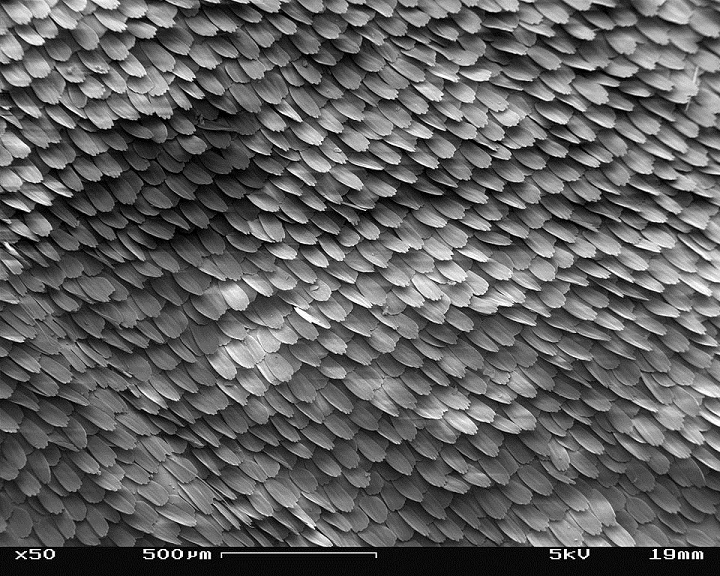
\includegraphics[width=\textwidth]{chapter_1/butterfly}
		\caption{Magnification 50x}
		\label{fig:b50}
	\end{subfigure}
	~ %add desired spacing between images, e. g. ~, \quad, \qquad, \hfill etc. 
	%(or a blank line to force the subfigure onto a new line)
	\begin{subfigure}[b]{0.3\textwidth}
		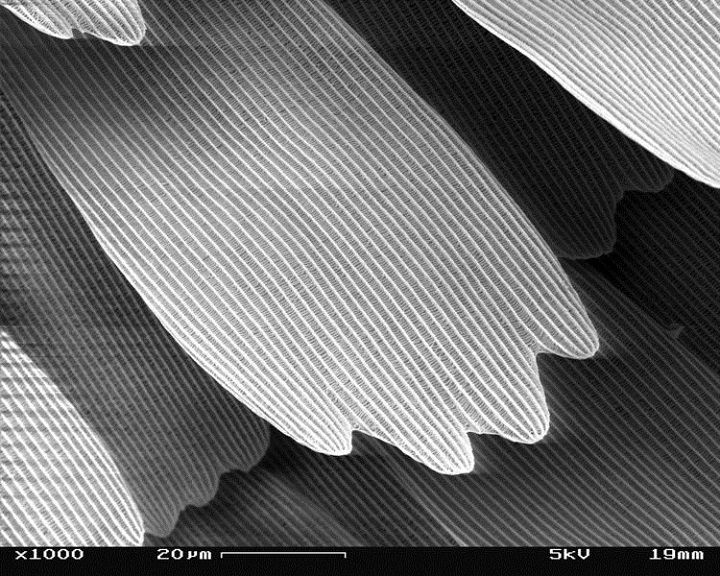
\includegraphics[width=\textwidth]{chapter_1/butterfly2}
		\caption{Magnification 1000x}
		\label{fig:b1000}
	\end{subfigure}
	~ %add desired spacing between images, e. g. ~, \quad, \qquad, \hfill etc. 
	%(or a blank line to force the subfigure onto a new line)
	\begin{subfigure}[b]{0.3\textwidth}
		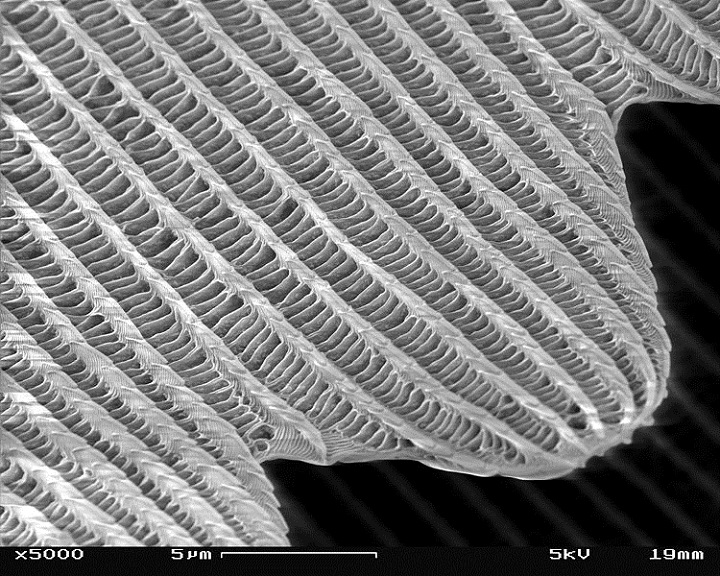
\includegraphics[width=\textwidth]{chapter_1/butterfly3}
		\caption{Magnification 5000x}
		\label{fig:b5000}
	\end{subfigure}
	\caption{Peacock butterfly wing surface using using Scanning Electron Microscopy.  Images from wikimedia.org}\label{fig:butterfly}
\end{figure}






\begin{figure}[h]
	\centering
	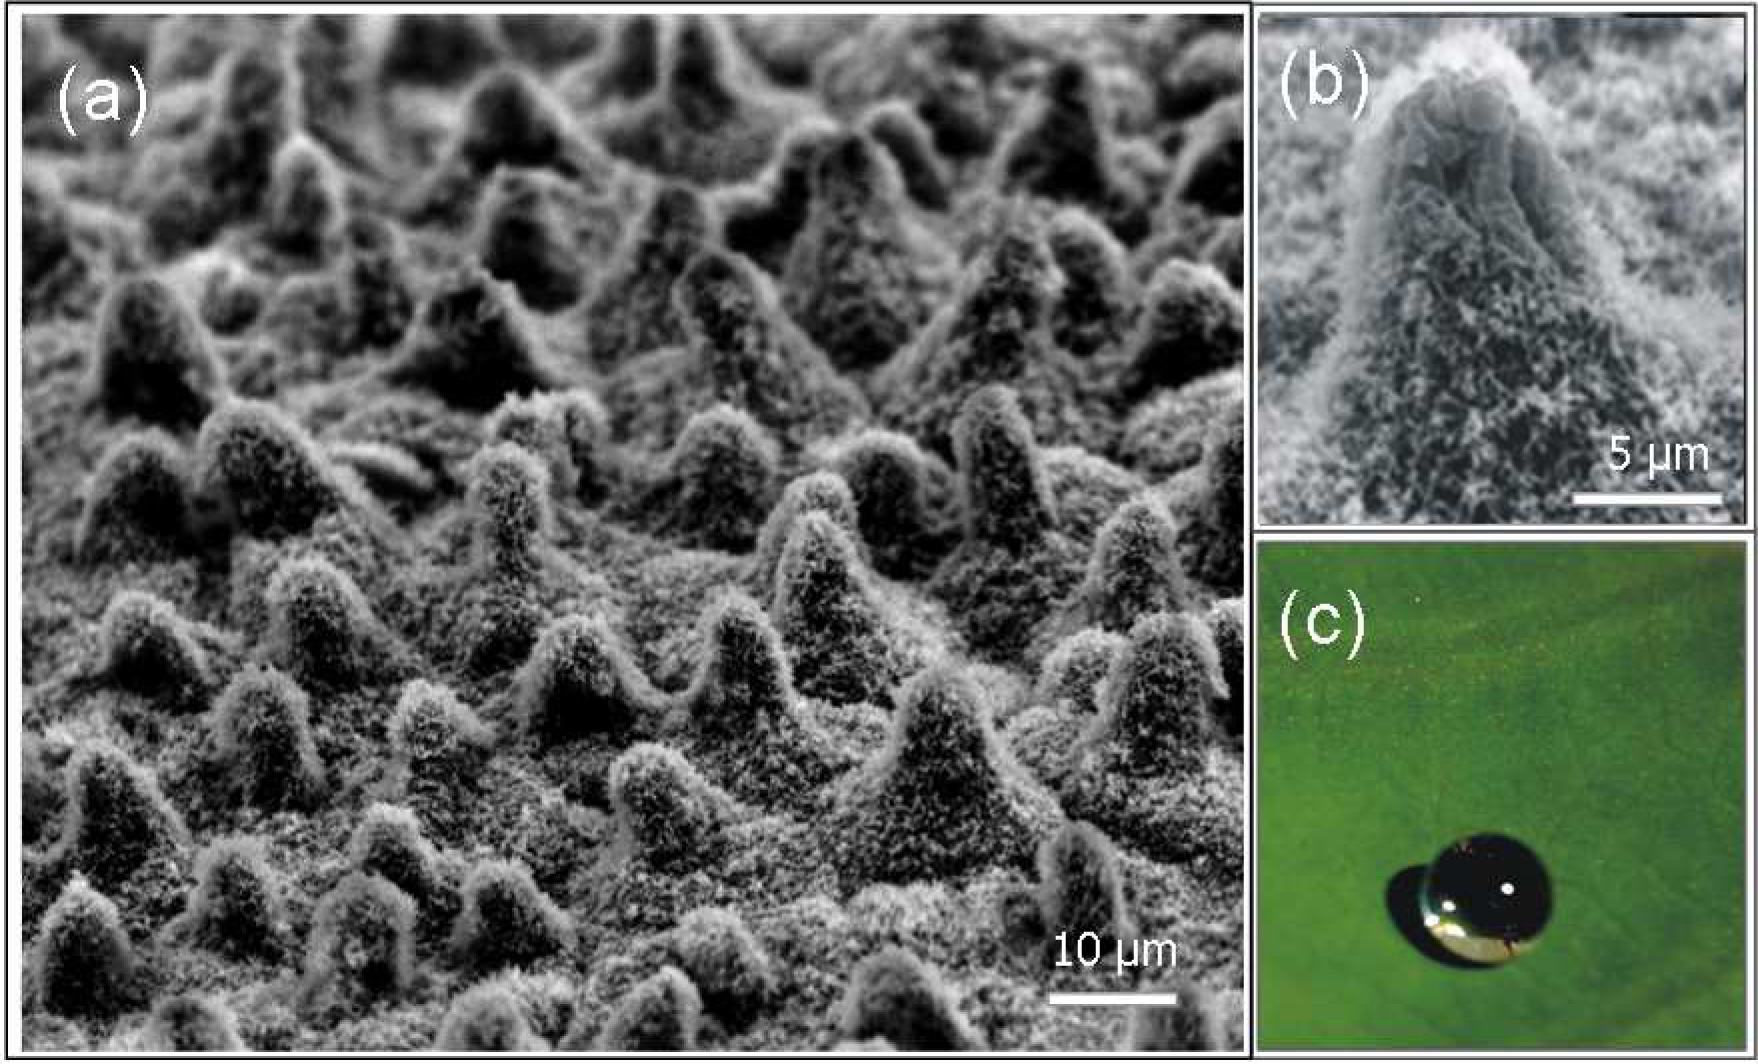
\includegraphics[width=0.5\linewidth]{chapter_1/lotus}
	\caption{(a) Lotus leaves, (b)(c) Scanning electron microscopy (SEM) images of the upper leaf side with different levels of magnification. Images from \cite{ensikat2011lotus}}
	\label{fig:lotus}
\end{figure}



\subsection{Riblets}

cita il paper con i riblets nel becco 